\documentclass{article}
\usepackage[utf8]{inputenc}
\usepackage{amsmath, amssymb, mathtools, graphicx, wrapfig}
\graphicspath{{Images/}}

\setlength{\oddsidemargin}{0in}
\setlength{\textwidth}{6.5in}
\setlength{\topmargin}{-.55in}
\setlength{\textheight}{9in}
\pagestyle{empty}

\title{Solid State Final}
\author{Michael Nameika}
\date{December 2022}

\begin{document}

\maketitle

\section*{Problem 1}
At what temperature $T_0$ does the specific heat of the free electrons become larger than the specific heat of the lattice? Express this temperature in terms of the Debye temperature and electron concentration. Calculate $T_0$ for copper using the following experimental facts: lattice constant $a = 0.365\text{nm}$, 1 electron goes to conducting band per atom, and $\Theta_D = 70^{\circ} \text{C}$.
\newline\newline
To begin, notice that $\Theta_D = 343.15 \text{K}$ and recall that the specific heat of free electrons is given by
\[C_{el} = \frac{1}{2}\pi^2N_{el}k_B\frac{T}{T_F}\]
and for the low temperature approximation, the specific heat of the lattice is given by
\[C_{lat} = \frac{12\pi^4}{5}N_{atoms}k_B\left(\frac{T}{\Theta_D}\right)^3\]
We wish to find $T$ such that $C_{el} \geq C_{lat}$. In particular, we want $T$ such that $C_el = C_{lat}$. Well,
\begin{align*}
    \frac{1}{2}\pi^2N_{el}k_B\frac{T}{T_F} &= \frac{12\pi^4}{5}N_{atoms}k_B\left(\frac{T}{\Theta_D}\right)^3 \\
    \frac{N_{el}}{N_{atoms}}T_F^{-1} &= \frac{24\pi^2}{5}\frac{T^2}{\Theta_D^3} \\
    T^2 &= \frac{5N_{el}T_F^{-1}\Theta_D^3}{24\pi^2N_{atoms}} \\
\end{align*}
Recall that the Fermi temperature $T_F$ is given by $\epsilon_F/k_B$, and in three dimensions, $\epsilon_F$ is given by
\[\epsilon_F = \frac{\hbar^2}{2m_{el}}\left(\frac{3\pi^2N_{el}}{V}\right)^{2/3}\]
So our above relationship becomes
\[T^2 = \frac{5N_{el}^{1/3}\Theta_D^3m_{el}k_BV^{2/3}}{12(\pi^2)^{5/3}\hbar^2N_{atoms}3^{2/3}}\]
Now, evaluating this temperature for copper, using $a = 3.65 \times 10^{-10} \text{ m}$, $\hbar = 1.055 \times 10^{-34} \text{ Js}$, $k_B = 1.381\times 10^{-23} \text{ JK}^{-1}$, $m_{el} = 9.109\times 10^{-31} \text{ kg}$, $N_{el} = N_{atoms} = 1$, we find 
\[T^2 \approx 105.12 \text{ K}\]
\[T \approx 10.25 \text{ K}\]
So at approximately $10.25 \text{ K}$ (and temperatures lower than this), we have that the specific heat of free electrons becomes larger than the specific heat of the lattice.

\section*{Problem 2}
Imagine that you were given a single monolayer of Cu atoms. These atoms are arranged like in a bulk Cu along [111] direction. What kin of symmetry do you have in this case? Using numerical values for bulk Cu lattice constant ($a = 0.361 \text{ nm}$) determine the 2-D lattice constant. Assuming that there is one electron per unit cell that is free to move in 2D plane, determine the value of Fermi energy in eV. If you replace Cu atoms with Pd atoms (bulk lattice constant is $a = 0.389 \text{ nm}$), how much will the Fermi level change? (Note that the assumption of one electron per unit cell for Cu is not correct, while for Pd is probably just fine. Nevertheless, use this assumption!)
\newline\newline
See attached sketches for details. Since Cu crystallizes in the FCC system, along the [111] direction, we have a 2-dimensional hexagonal lattice. Then the lattice constant for the [111] layer of Cu will be given by
\[\frac{1}{\sqrt{2}}a = \frac{1}{\sqrt{2}}(0.361 \text{ nm}) \approx 0.2553 \text{ nm}\]
From the Schr\"odinger equation, we can expect to find energy eigenvalues of the form
\[\frac{h^2}{2m_{el}}k_F^2\]
Then for the number of electrons inside a Fermi 2-sphere of radius $k_F$, we have
\[N_{el} = 2\frac{\pi k_F^2}{(2\pi/L)^2} = \frac{Ak_F^2}{2\pi}\]
so
\[k_F^2 = \frac{2\pi N_{el}}{A}\]
so our Fermi energy takes the form
\[\epsilon_F = \frac{\hbar^2\pi N_{el}}{Am_{el}}\]
And the area of our primitive 2-D hexagonal lattice is 
\[A = \frac{\sqrt{3}}{4}a^2\]
Using this in our equation for Fermi energy, we find for one electron in the unit cell,
\[\epsilon_F \approx 0.42 \text{ keV}\]
Finally, since Pd also crystallizes in the FCC lattice, we have the same 2-D lattice in the [111] direction, so using the value $a = 0.389 \text{ nm}$, we find the following for the Fermi energy for one electron in the unit cell:
\[\epsilon_F \approx 0.365 \text{ keV}\]

\newpage
\section*{Problem 3}
\begin{wrapfigure}{r}{0.25\textwidth}
    \begin{center}
        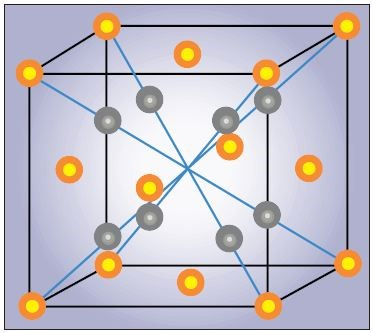
\includegraphics[width = 0.30\textwidth]{lattice.jpg}
    \end{center}
\end{wrapfigure}
The image below illustrates the $\text{CaF}_2$ structure. The lattice constant, $a$, for this compound is $5.462 \: \AA$. 
(a) At what angle $\Theta$ will the reflection from crystallographic planes in the XRD experiment occur if you will use Cu radiation ($\lambda = 0.15406 \text{ nm}$). 
(b) Calculate the structural factor for the first 10 nonvanishing peaks. 
Assume that the ratio of atomic scattering factors ($f_{\text{Ca}}/f_{\text{F}}$) is like 2:1 (In reality it is 1.8 and their values are changing with $\Theta$ - neglect this fact! 
For this reason, your calculated result will be different from experimental results).
Comment on the intensity of the peaks.
\newline\newline
To find the allowed values of $\Theta$, we will use Bragg's law of diffraction:
\[n\lambda = 2d\sin(\Theta)\]
in this case we will use $n = 1$ and recall that
\[d = \frac{a}{\sqrt{h^2 + k^2 + l^2}}\]
where $h,k,l$ are the miller indices of a crystal plane.
Solving for $\Theta$, we find
\[\Theta = \arcsin\left(\frac{0.15406}{2(0.5462)}\sqrt{h^2 + k^2 + l^2}\right)\]
then the allowed values for $\Theta$ are 
\begin{center}
    \begin{tabular}{c|c|c}
        $8.107^{\circ}$ & $34.341^{\circ}$ & $52.918^{\circ}$ \\
        $11.505^{\circ}$ & $35.552^{\circ}$ & $54.111^{\circ}$ \\
        $14.139^{\circ}$ & $36.750^{\circ}$ & $55.319^{\circ}$ \\
        $16.381^{\circ}$ & $37.930^{\circ}$ & $56.545^{\circ}$ \\
        $18.380^{\circ}$ & $39.102^{\circ}$ & $57.800^{\circ}$ \\
        $20.208^{\circ}$ & $40.261^{\circ}$ & $60.384^{\circ}$ \\
        $23.508^{\circ}$ & $41.413^{\circ}$ & $64.561^{\circ}$ \\
        $25.030^{\circ}$ & $43.699^{\circ}$ & $66.060^{\circ}$ \\
        $26.486^{\circ}$ & $44.839^{\circ}$ & $67.638^{\circ}$ \\
        $27.886^{\circ}$ & $45.981^{\circ}$ & $71.093^{\circ}$ \\
        $29.244^{\circ}$ & $47.122^{\circ}$ & $77.710^{\circ}$ \\
        $30.562^{\circ}$ & $49.415^{\circ}$ & $85.731^{\circ}$ \\
        $31.849^{\circ}$ & $50.574^{\circ}$ &  \\
    \end{tabular}
\end{center}
Now, to evaluate the structure factor, notice from the figure that the crystal appears to be an FCC lattice with an embedded simple cubic lattice. Since there are more fluorine atoms in the crystal than calcium, I will assume that the yellow atoms are fluorine and the grey atoms are calcium. From this, we have that there will be 4 fluorine atoms per basis and 1 calcium atom per basis. Then our fluorine basis atoms will be located at $(0,0,0)$, $(1/2,1/2,0)$, $(1/2,0,1/2)$, and $(0,1/2,1/2)$ and our calcium basis atom will be located at $(1/4,1/4,1/4)$ since it is a quarter of the way up the main diagonal. Then our structure factor becomes
\[S = f\left(1 + e^{-i\pi(v_1 + v_2)} + e^{-i\pi(v_1 +v_3)} + e^{-i\pi(v_2 + v_3)} + 2e^{-i\pi/2(v_1 + v_2 + v_3)}\right)\]
evaluating for the first 10 nonvanishing peaks, we find the following:
\begin{center}
    \begin{tabular}{c|c|c}
        $(hkl)$ & $S$ & $|S|$ \\
        \hline
        (100) & $-2if$ & $2f$ \\
        (110) & $-2f$ & $2f$ \\
        (111) & $(4 + 2i)f$ & $2\sqrt{5}f$ \\
        (200) & $2f$ & $2f$ \\
        (210) & $2if$ & $2f$ \\
        (211) & $2f$ & $2f$ \\
        (220) & $6f$ & $6f$ \\
        (221) & $-2if$ & $2f$ \\
        (222) & $2f$ & $2f$ \\
        (300) & $2if$ & $2f$ \\
    \end{tabular}
\end{center}
So most peaks have an intensity of $2f$, with a couple of sharper peaks of intensity $6f$ and $2\sqrt{5}f \approx 4.47f$.

\section*{Problem 4}
Evaluate the Fermi function for an energy $kT$ above the Fermi energy. (b) Find the temperature at which there is a 1\% probability that a state, with an energuy 0.5 eV above the Fermi energy, will be occupied by the electron. ($k_B = 1.3807\times 10^{-23} \text{ j/K}$)
\newline\newline
Recall the general form for the Fermi function:
\[f(\epsilon) = \frac{1}{\exp{\left[(\epsilon - \mu)/k_BT\right]} + 1}\]
Then for an energy $k_BT$ above the Fermi energy, $\epsilon = \epsilon_F + k_BT$ and
\begin{align*}
    f(\epsilon_F + k_BT) &= \frac{1}{\exp{[(\epsilon_F + k_BT - \mu)/k_BT]} + 1} \\
    &= \frac{1}{\exp{[(\epsilon_F - \mu)/k_BT + 1]} + 1} \\
\end{align*}
Now we wish to find the temperature at which there is a 1\% probability that a state with energy 0.5 eV above the Fermi energy will be occupied by the electron. That is, we must solve the following equation for $T$:
\begin{align*}
    f(\epsilon_F + 0.5 \text{ eV}) &= \frac{1}{\exp{[(\epsilon_f - \mu)/k_BT + (0.5 \text{ eV})/k_BT]} + 1} = 0.01 \\
\end{align*}
Recall that we may approximate $\mu$ as
\[\mu \approx \epsilon_F \left[1 - \frac{\pi^2}{12}\left(\frac{k_BT}{\epsilon_F}\right)^2\right]\]
Then
\[\frac{\epsilon_F - \mu}{k_BT} \approx \frac{\pi^2}{12}\left(\frac{k_BT}{\epsilon_F}\right)\]
Using this and rearranging the above equation for our Fermi probability, we find
\begin{align*}
    \exp{\left[\frac{\pi^2}{12}\left(\frac{T}{T_F}\right) + \frac{0.5 \text{ eV}}{k_BT}\right]} + 1&= 100 \\
    \frac{\pi^2}{12}\left(\frac{T}{T_F}\right) + \frac{0.5 \text{ eV}}{k_BT} &= \ln{(99)} \\
    \frac{\pi^2}{12}\frac{T^2}{T_F} - T\ln{(99)} + \frac{0.5 \text{ eV}}{k_B} &= 0 \\
\end{align*}
Using the quadratic formula, we find the following expression for $T$:
\[T = \frac{\ln{(99)} + \sqrt{(\ln{(99)})^2 - \pi^2(0.5 \text{ eV})/(3T_Fk_B)}}{\pi^2/(6T_F)}\]
where $T_F$ is the Fermi temperature.

\section*{Problem 5}
I will ask two of my students, Sara and Paul, to prepare for you a set of samples made out of metal (for example, Cu - this would be Sara's task) and semiconductor (made by Paul) in the form of patterned films. These samples will be grown on MgO substrates. Each of them will prepare two samples of thicknesses $d = 100 \; \mu\text{m}$ and 100 nm. We know that the concentration of electrons in a metal is on the order of $10^{22} \text{ cm}^{-3}$ while in semiconductor (n-type) it is on the order of $10^{14} \text{ cm}^{-3}$. In the experiment, we will use a current source that will deliver a current of 10 mA. These samples will be placed in the magnetic field ($B = 0.1 \text{ T}$). Determine the magnitude of the Hall voltage ($V_H$) in these samples. How easily can we measure such voltages? If we would use any metal, will the sign of the Hall voltage be the same as for the considered semiconductor?
\newline\newline
Recall that hall voltage is related to current, magnetic field, and thickness of a sample by
\[V_H = -\frac{B_0I}{ane}\]
where $n$ is the charge carrier density, $e$ is the elementary charge, and $a$ is the thickness of the sample. For this problem, we are given $a_{metal} = 100 \; \mu\text{m}$ and $B = 0.1 \text{ T}$, $n_{metal} = 10^{22} \text{ cm}^{-3}$, so the magnitude of the Hall voltage for the metal is given by
\begin{align*}
    |V_{H,metal}| &= \frac{(0.1 \text{ Vs/m})(10^{-2} \text{ C/s})}{(10^{-4} \text{ m})(10^{28} \text{ m}^{-3})(1.602 \times 10^{-19} \text{ C})} \\
    &\approx 6.42 \times 10^{-9} \text{ V} \\
\end{align*}
And the magnitude of the Hall voltage for the semiconductor is given by
\begin{align*}
    |V_{H,sc}| &= \frac{(0.1 \text{ Vs/m})(10^{-2} \text{ C/s})}{(10^{-7} \text{ m})(10^{20} \text{ m}^{-3})(1.602\times 10^{-19 \text{ C}})} \\
    &\approx 624.22 \text{ V} \\
\end{align*}
The Hall voltage on the metal will likely be very difficult to detect, though likely not impossible, and the Hall voltage on the semiconductor will easily be detected. If we were to use any metal, the sign of the Hall voltage likely won't be the same as the sign of the Hall voltage for the semiconductor, since some metals have a measured Hall coefficient that is opposite sign from the theoretical Hall coefficient.

\end{document}

